\documentclass[margin=10pt]{standalone}
\usepackage{cmbright}
%\renewcommand{\familydefault}{\sfdefault}
%
\usepackage{tikz}
\usetikzlibrary{arrows}
\usetikzlibrary{arrows.meta}
\usetikzlibrary{backgrounds}
\usetikzlibrary{decorations.markings}
\usetikzlibrary{fit}
\usetikzlibrary{matrix}
\usetikzlibrary{positioning}
\usetikzlibrary{shadows}

\begin{document}
{
\normalsize
%\large

\newsavebox\mybox
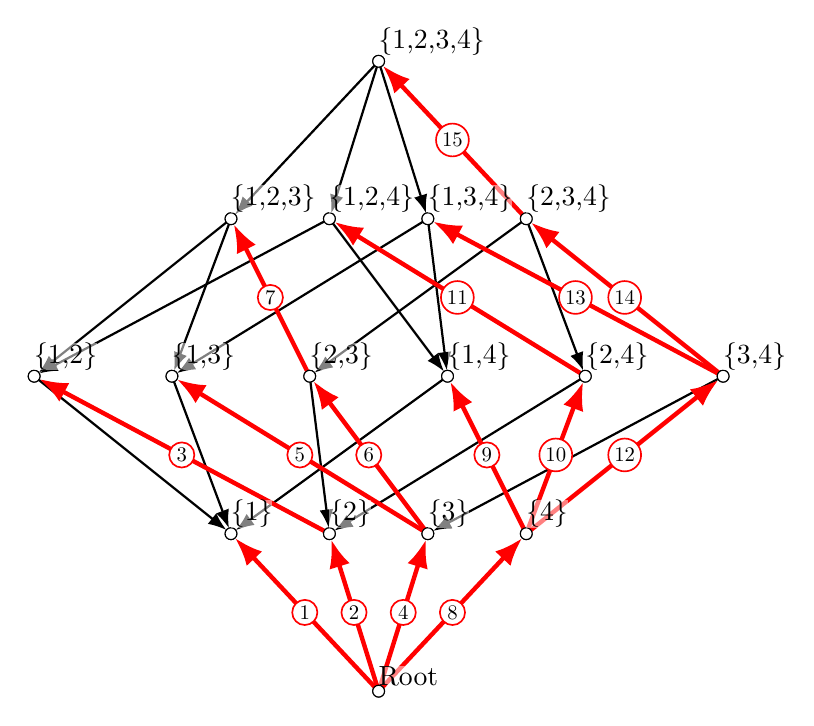
\begin{tikzpicture}[
		every node/.style = {
			draw,
			fill = white!5,
			align = center,
		},
		labeltxt/.style = {
			draw = none,
			fill = white,
			fill opacity = 0.5,
			text opacity = 1,
			anchor = south west,
			outer sep = 0,
			inner sep = 0,
		},
		line/.style = {
			ultra thick,
		},
		point/.style = {
			%fill=black,
			inner sep = 0pt,
			outer sep = 0pt,
			minimum size = 1.5mm, 
			circle,
		},
		bgbox/.style = {
			densely dotted,
			rounded corners,
			fill = black!10,
			%drop shadow,
		},
		uparr/.style = {
			ultra thick,
			draw = red,
        	-Latex,
        },
        downarr/.style = {
			thick,
        	-Latex,
        },
        arrlbl/.style={
            scale = 0.75,
        	circle,
        	semithick,
			inner sep = 0.05 cm,
        },
 		]

	%\draw[step=1cm,black!80,very thin] (0,0) grid (15,15);
	%\draw[step=0.5cm,black!20,very thin] (0,0) grid (15,15);

	\pgfmathsetlengthmacro{\base}{6cm};
	\pgfmathsetlengthmacro{\vb}{0cm};
	\pgfmathsetlengthmacro{\vo}{2cm};
	\pgfmathsetlengthmacro{\ho}{1.25cm};

	% TETRAHEDRON
	\coordinate[point] (4n) at (\base,\vb);

	\coordinate[point] (41a) at (\base-1.5*\ho,\vb+\vo);
	\coordinate[point] (41b) at (\base-\ho/2,\vb+\vo);
	\coordinate[point] (41c) at (\base+\ho/2,\vb+\vo);
	\coordinate[point] (41d) at (\base+1.5*\ho,\vb+\vo);

	\pgfmathsetlengthmacro{\ho}{1.75cm};
	\coordinate[point] (42a) at (\base-2.5*\ho, \vb+2*\vo);
	\coordinate[point] (42b) at (\base-1.5*\ho, \vb+2*\vo);
	\coordinate[point] (42c) at (\base-\ho/2, \vb+2*\vo);
	\coordinate[point] (42d) at (\base+\ho/2,\vb+2*\vo);
	\coordinate[point] (42e) at (\base+1.5*\ho,\vb+2*\vo);
	\coordinate[point] (42f) at (\base+2.5*\ho,\vb+2*\vo);

	\pgfmathsetlengthmacro{\ho}{1.25cm};
	\coordinate[point] (43a) at (\base-1.5*\ho,\vb+3*\vo);
	\coordinate[point] (43b) at (\base-\ho/2,\vb+3*\vo);
	\coordinate[point] (43c) at (\base+\ho/2,\vb+3*\vo);
	\coordinate[point] (43d) at (\base+1.5*\ho,\vb+3*\vo);

	\coordinate[point] (44) at (\base,\vb+4*\vo);



	\draw[downarr] (42a) -- (41a);
	\draw[downarr] (42b) -- (41a);
	\draw[downarr] (42c) -- (41b);
	\draw[downarr] (42d) -- (41a);
	\draw[downarr] (42e) -- (41b);
	\draw[downarr] (42f) -- (41c);

	\draw[downarr] (43a) -- (42a);
	\draw[downarr] (43a) -- (42b);
	\draw[downarr] (43b) -- (42a);
	\draw[downarr] (43b) -- (42d);
	\draw[downarr] (43c) -- (42b);
	\draw[downarr] (43c) -- (42d);
	\draw[downarr] (43d) -- (42c);
	\draw[downarr] (43d) -- (42e);

	\draw[downarr] (44) -- (43a);
	\draw[downarr] (44) -- (43b);	
	\draw[downarr] (44) -- (43c);


	\draw[uparr] (4n) -- node[arrlbl]{1} (41a);
	\draw[uparr] (4n) -- node[arrlbl]{2} (41b);
	\draw[uparr] (41b) -- node[arrlbl]{3} (42a);
	\draw[uparr] (4n) -- node[arrlbl]{4} (41c);
	\draw[uparr] (41c) -- node[arrlbl]{5} (42b);
	\draw[uparr] (41c) -- node[arrlbl]{6} (42c);
	\draw[uparr] (42c) -- node[arrlbl]{7} (43a);
	\draw[uparr] (4n) -- node[arrlbl]{8} (41d);
	\draw[uparr] (41d) -- node[arrlbl]{9} (42d);
	\draw[uparr] (41d) -- node[arrlbl]{10} (42e);
	\draw[uparr] (42e) -- node[arrlbl]{11} (43b);
	\draw[uparr] (41d) -- node[arrlbl]{12} (42f);
	\draw[uparr] (42f) -- node[arrlbl]{13} (43c);
	\draw[uparr] (42f) -- node[arrlbl]{14} (43d);
	\draw[uparr] (43d) -- node[arrlbl]{15} (44);


	\coordinate[point, label={[labeltxt]:Root}] (4n) at (\base,\vb);

	\coordinate[point, label={[labeltxt]:\{1\}}] (41a) at (\base-1.5*\ho,\vb+\vo);
	\coordinate[point, label={[labeltxt]:\{2\}}] (41b) at (\base-\ho/2,\vb+\vo);
	\coordinate[point, label={[labeltxt]:\{3\}}] (41c) at (\base+\ho/2,\vb+\vo);
	\coordinate[point, label={[labeltxt]:\{4\}}] (41d) at (\base+1.5*\ho,\vb+\vo);

	\pgfmathsetlengthmacro{\ho}{1.75cm};
	\coordinate[point, label={[labeltxt]:\{1,2\}}] (42a) at (\base-2.5*\ho, \vb+2*\vo);
	\coordinate[point, label={[labeltxt]:\{1,3\}}] (42b) at (\base-1.5*\ho, \vb+2*\vo);
	\coordinate[point, label={[labeltxt]:\{2,3\}}] (42c) at (\base-\ho/2, \vb+2*\vo);
	\coordinate[point, label={[labeltxt]:\{1,4\}}] (42d) at (\base+\ho/2,\vb+2*\vo);
	\coordinate[point, label={[labeltxt]:\{2,4\}}] (42e) at (\base+1.5*\ho,\vb+2*\vo);
	\coordinate[point, label={[labeltxt]:\{3,4\}}] (42f) at (\base+2.5*\ho,\vb+2*\vo);

	\pgfmathsetlengthmacro{\ho}{1.25cm};
	\coordinate[point, label={[labeltxt]:\{1,2,3\}}] (43a) at (\base-1.5*\ho,\vb+3*\vo);
	\coordinate[point, label={[labeltxt]:\{1,2,4\}}] (43b) at (\base-\ho/2,\vb+3*\vo);
	\coordinate[point, label={[labeltxt]:\{1,3,4\}}] (43c) at (\base+\ho/2,\vb+3*\vo);
	\coordinate[point, label={[labeltxt]:\{2,3,4\}}] (43d) at (\base+1.5*\ho,\vb+3*\vo);

	\coordinate[point, label={[labeltxt]:\{1,2,3,4\}}] (44) at (\base,\vb+4*\vo);

\end{tikzpicture}
}% end size


\end{document}   